\subsection{Resoluci\'on}

En nuestra heuristica de busqueda local decidimos tomar la solucion desde la que partimos y mejorarla tomando el primer nodo $nodo1$ y moviendolo a otro conjunto, verificando aqui si la solucion del peso total de todos los conjuntos mejora o empeora (tomandonos la libertad de decir que empeora aun si el peso total es el mismo). Si empeora continuamos de la solucion que ya teniamos tomando el proximo nodo, $nodo2$ y repitiendo el mismo proceso de probarlo el los demas conjuntos. En caso de que la solucion mejore guardamos el nodo que genera esta mejora y el conjunto al que se deberia mover. Una vez que se realizo este proceso en todos los nodos terminaremos teniendo una solucion mejor o en el peor caso la misma con la que empezamos.
Si la solución pudo ser mejorada, tomamos esta y se vuelve a ejecutar este procedimiento para esta nueva solucion hasta que se llegue a una solucion que no puede ser mejorada (mediante esta heuristica).
Como se puede notar para cada solucion factible definimos el conjunto de soluciones "vecinas" como: aquellas en las que difiere la posicion de un solo nodo sobre los k conjuntos, iterando sobre estas hasta hallar la mejora de forma mayoritaria la solucion. Esto se repite hasta que se encuentra un valor maximo local (maximo en cuanto a la optimalidad de la solucion) que corresponde al minimo peso obtenido.

Pensamos tambien plantear la misma solucion cambiando la vecindad de soluciones, en esta nueva heuristica en lugar de verificar

A modo de ejemplo presentamos una demostracion grafica de la heuristica.


Partimos de la siguiente solucion (1)
\begin{figure}[H]
\begin{center}
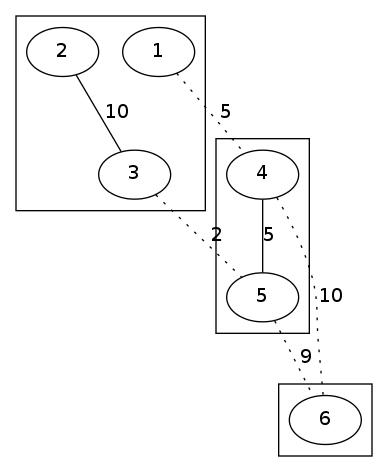
\includegraphics[scale=0.4]{./img/local1.png}
\caption{(1) Solución inicial con k=3}
\end{center}
\end{figure}

A partir de ahora verificara si moviendo un nodo de conjunto puede llegar a una mejor solución, en este momento la suma de los pesos de las aristas intraparticion es igual a 15. Moviendo el nodo $1$ a cualquiera de los otros dos conjuntos no se logra disminuir el peso total, por lo que queda donde esta, ahora el nodo $2$ logra disminuir en 10 moviendolo a cualquiera de los dos conjuntos restantes, se decide moverlo al segundo. (2)

\begin{figure}[H]
\begin{center}
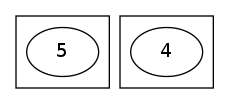
\includegraphics[scale=0.4]{./img/greedy2.png}
\caption{(2) Solución vecina habiendo movido el nodo $2$}
\end{center}
\end{figure}


Ahora el nodo $3$ aumenta el peso total si se mueve al siguiente conjunto y no aporta nada moverlo al ultimo, por lo que queda en el conjunto en el que está. Lo mismo pasa con el nodo $4$, moviendolo a uno aumenta el peso y al otro se mantiene. Sigue el nodo $5$ que si se mueve al conjunto donde están los nodos $1$ y $3$ disminuye el peso total a 2, y si se mueve al conjunto restante aumenta el peso en 5, por lo que se ubica en el primer conjunto. Finalmente el nodo $6$ no produce cambios de peso favorables moviendolo, por lo que la solución a la que llega la heuristica es la de la figura (3).

\begin{figure}[H]
\begin{center}
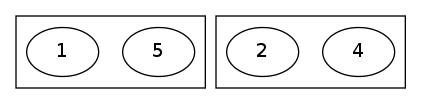
\includegraphics[scale=0.4]{./img/greedy3.png}
\caption{(3) Solución vecina habiendo movido el nodo $5$ a partir de la solucion (2).}
\end{center}
\end{figure}

Habiendo encontrado la solucion (3) se llama al recursivamente y se vuelve a realizar el mismo procedimiento. En este caso los nodos $1$, $2$, $3$ y $4$ no mejoran el peso moviendose de donde están, en cambio el nodo $5$ logra encontrar un peso menor moviendose al conjunto donde se encuentra el nodo $6$ siendo este cero. Al encontrar una solucion optima ningun movimiento podrá mejorarla, razon por la cual la solucion final es la que muestra la imagen (4). 

\begin{figure}[H]
\begin{center}
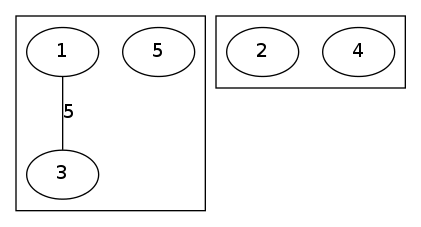
\includegraphics[scale=0.4]{./img/greedy4.png}
\caption{(4) Solución máxima local.}
\end{center}
\end{figure}

A continuación presentamos un pseudo-grafico del algoritmo realizado:

\begin{itemize}
\item RESOLVER
	\begin{itemize}
	\item Para cada vertice $v$
		\begin{itemize}
		\item Para cada particion $p$
			\begin{itemize}
			\item Si $v$ esta en la particion $k$, Se calcula cuanto peso 'perdería' restando las aristas intraparticion que inciden en $k$
			\item Sino se calcula cuanto peso 'sumaria' mover $v$ a $p$ guardando el peso, $v$ y $p$ si suma menos peso que con los $v$ y $p$ anteriores.
			\end{itemize}
		\item Si se llego a una solucion mejor, se guarda
		\end{itemize}
	\item Si se encontró alguna solución mejor a la inicial se la toma y se llama recursivamente a RESOLVER con esta.
	\end{itemize}
\end{itemize}




